\documentclass[12pt,a4paper]{article}

% Packages
\usepackage[utf8]{inputenc}
\usepackage[portuguese]{babel}
\usepackage{graphicx}
\usepackage{geometry}
\usepackage{hyperref}
\usepackage{listings}
\usepackage{xcolor}
\usepackage{float}
\usepackage{amsmath}

% Page geometry
\geometry{
    top=2.5cm,
    bottom=2.5cm,
    left=2.5cm,
    right=2.5cm
}

% Hyperref setup
\hypersetup{
    colorlinks=true,
    linkcolor=black,
    urlcolor=blue,
    citecolor=black
}

% Code listings setup
\lstset{
    language=Python,
    basicstyle=\ttfamily\small,
    keywordstyle=\color{blue},
    commentstyle=\color{green!60!black},
    stringstyle=\color{red},
    showstringspaces=false,
    breaklines=true,
    frame=single,
    numbers=left,
    numberstyle=\tiny\color{gray},
    captionpos=b,
    tabsize=4
}

\begin{document}

% Title page
\begin{titlepage}
    \centering
    
    \vspace*{0.8cm}
    
    {\Large Instituto Superior de Engenharia de Lisboa}\\[0.3cm]
    {\large Departamento de Engenharia Eletrónica e Telecomunicações e de Computadores (DEETC)}\\[0.3cm]
    {\large Mestrado em Engenharia Informática e de Computadores}\\[2cm]
    
    {\huge\bfseries Módulo de Prática \#06}\\[0.3cm]
    {\LARGE Avaliação de Modelos}\\[1.5cm]
    
    {\Large Aprendizagem e Mineração de Dados (AMD)}\\[0.3cm]
    {\large 1º Semestre -- 2025/2026}\\[3cm]

    
\includegraphics[width=0.8\textwidth]{figures/01_ISEL-Logotipo-RGB_Horizontal-Compacto-900.png}\\[0.8cm]
    
    {\large \textbf{Autores:}}\\[0.3cm]
    {\large Florin Sofinet (A46608)}\\[0.2cm]
    {\large Diogo Guerra (A49149)}\\[0.2cm]
    {\large Nuno Silva (A53976)}\\[2cm]
    
    {\large \today}
    
    \vfill
    
\end{titlepage}

\newpage
\tableofcontents
\newpage

\section{Introdução}

Este laboratório tem como objetivo explorar métodos de avaliação de modelos de Machine Learning, combinando capacidades programáticas de Python com ferramentas de outras bibliotecas e do ambiente do Orange Data Mining.

Ao longo do trabalho, serão analisadas diversas técnicas de divisão de dados, métodos de amostragem, bootstrap, métricas de desempenho e construção de classificadores.

Os objetivos principais são:
\begin{enumerate}
    \item Integrar bibliotecas Python no ambiente Orange Data Mining
    \item Carregar e processar datasets para análise
    \item Compreender e implementar métodos de divisão treino-teste (holdout, stratified holdout, holdout repetido)
    \item Implementar e analisar métodos avançados de amostragem (leave-one-out, leave-p-out, k-fold, bootstrap)
    \item Construir classificadores utilizando scikit-learn
    \item Implementar múltiplas métricas de avaliação (exatidão, precisão, revocação, F1-score, Kappa de Cohen)
    \item Analisar avisos de métricas e compreender as suas causas
    \item Comparar desempenho em conjuntos de dados de diferentes tamanhos
\end{enumerate}

\section{Orange Data Mining}

\subsection{Objetivo}

Integrar a biblioteca pandas no ambiente virtual do Orange Data Mining para preparar o ambiente de trabalho necessário para os exercícios seguintes.

\subsection{1.a) Instalação da biblioteca pandas}

Foi instalada a biblioteca pandas no ambiente virtual do Orange utilizando o gestor de pacotes pip. Esta biblioteca é essencial para manipulação e análise de dados tabulares.

\subsection{1.b) Verificação das versões das bibliotecas}

Verificamos as versões das bibliotecas instaladas no ambiente virtual:
\begin{itemize}
    \item \textbf{pandas:} Biblioteca para manipulação de dados
    \item \textbf{numpy:} Biblioteca para computação numérica
    \item \textbf{scikit-learn:} Biblioteca para machine learning
\end{itemize}

Esta verificação garante que todas as dependências necessárias estão corretamente instaladas e com versões compatíveis para os exercícios seguintes.

\begin{figure}[H]
\centering
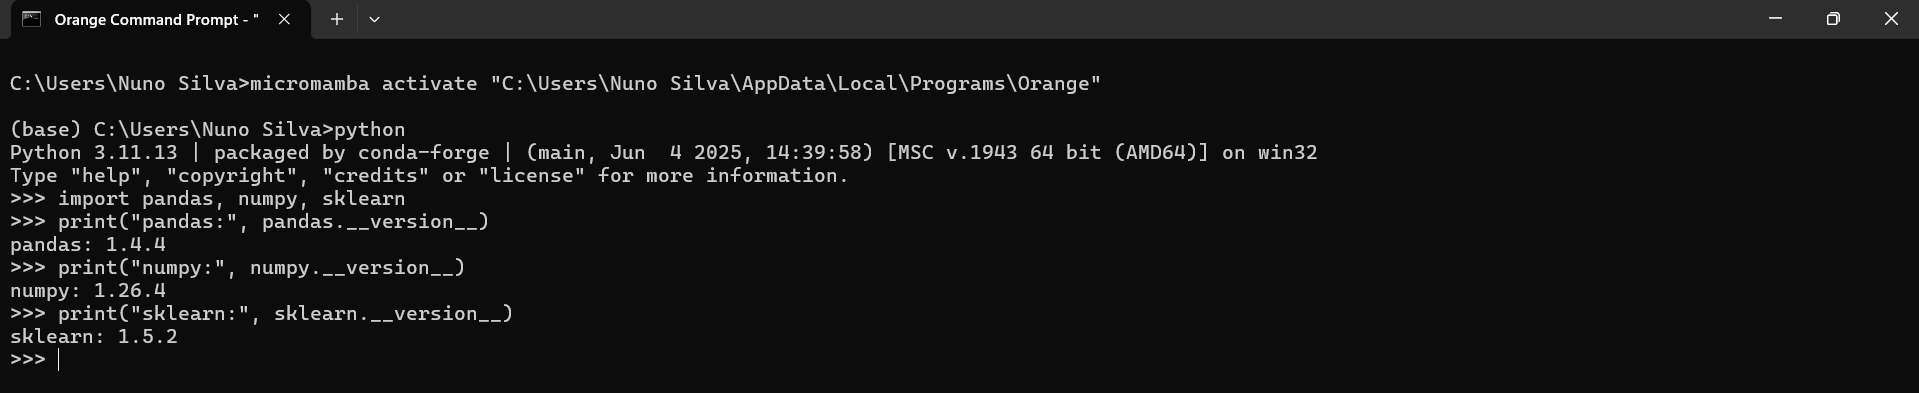
\includegraphics[width=0.8\textwidth]{figures/verificacao_versoes.png}
\caption{Verificação das versões de pandas, numpy e scikit-learn instaladas no ambiente virtual}
\end{figure}

\section{Carregamento de um Dataset}

\subsection{Objetivo}

Compreender como os datasets são lidos, processados e disponibilizados para análise através de diferentes métodos de carregamento.

\subsection{2.a) Execução do ficheiro original}

Executamos o ficheiro \texttt{my\_split\_and\_eval.py} original sem alterações para compreender o comportamento padrão do script e verificar o seu correto funcionamento.

\begin{figure}[H]
\centering
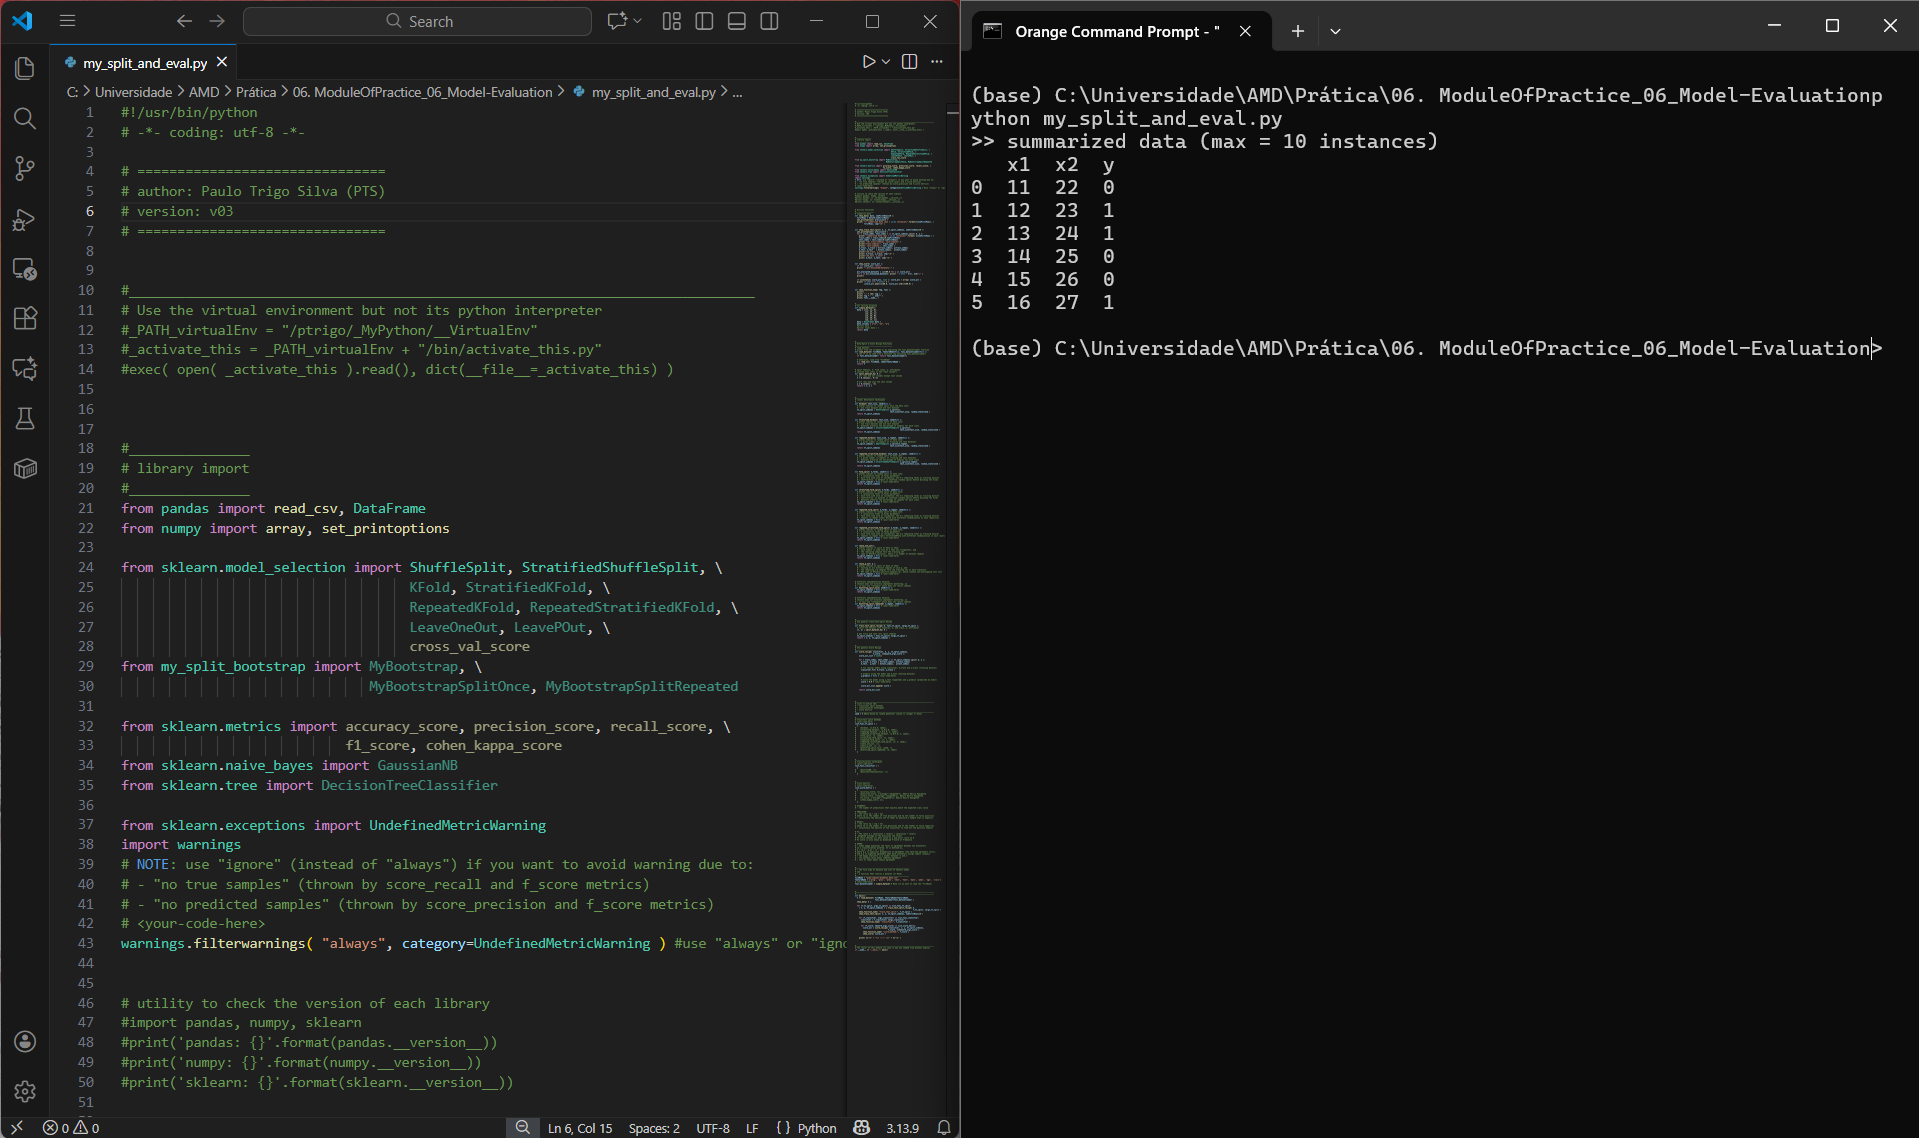
\includegraphics[width=0.9\textwidth]{figures/execucao_my_split_and_eval.png}
\caption{Execução do ficheiro my\_split\_and\_eval.py sem alterações}
\end{figure}

\subsection{2.b) Carregamento do dataset Pima Indians Diabetes}

Substituímos a função de carregamento do \texttt{simple\_dataset} pelo carregamento direto do ficheiro \texttt{pima-indians-diabetes.data.csv}.

Este dataset contém:
\begin{itemize}
    \item \textbf{Instâncias:} 768 pacientes
    \item \textbf{Características:} 8 características médicas (gravidez, glucose, pressão arterial, espessura da pele, insulina, IMC, pedigree de diabetes, idade)
    \item \textbf{Classes:} 2 (diabético vs. não-diabético)
\end{itemize}

\begin{figure}[H]
\centering
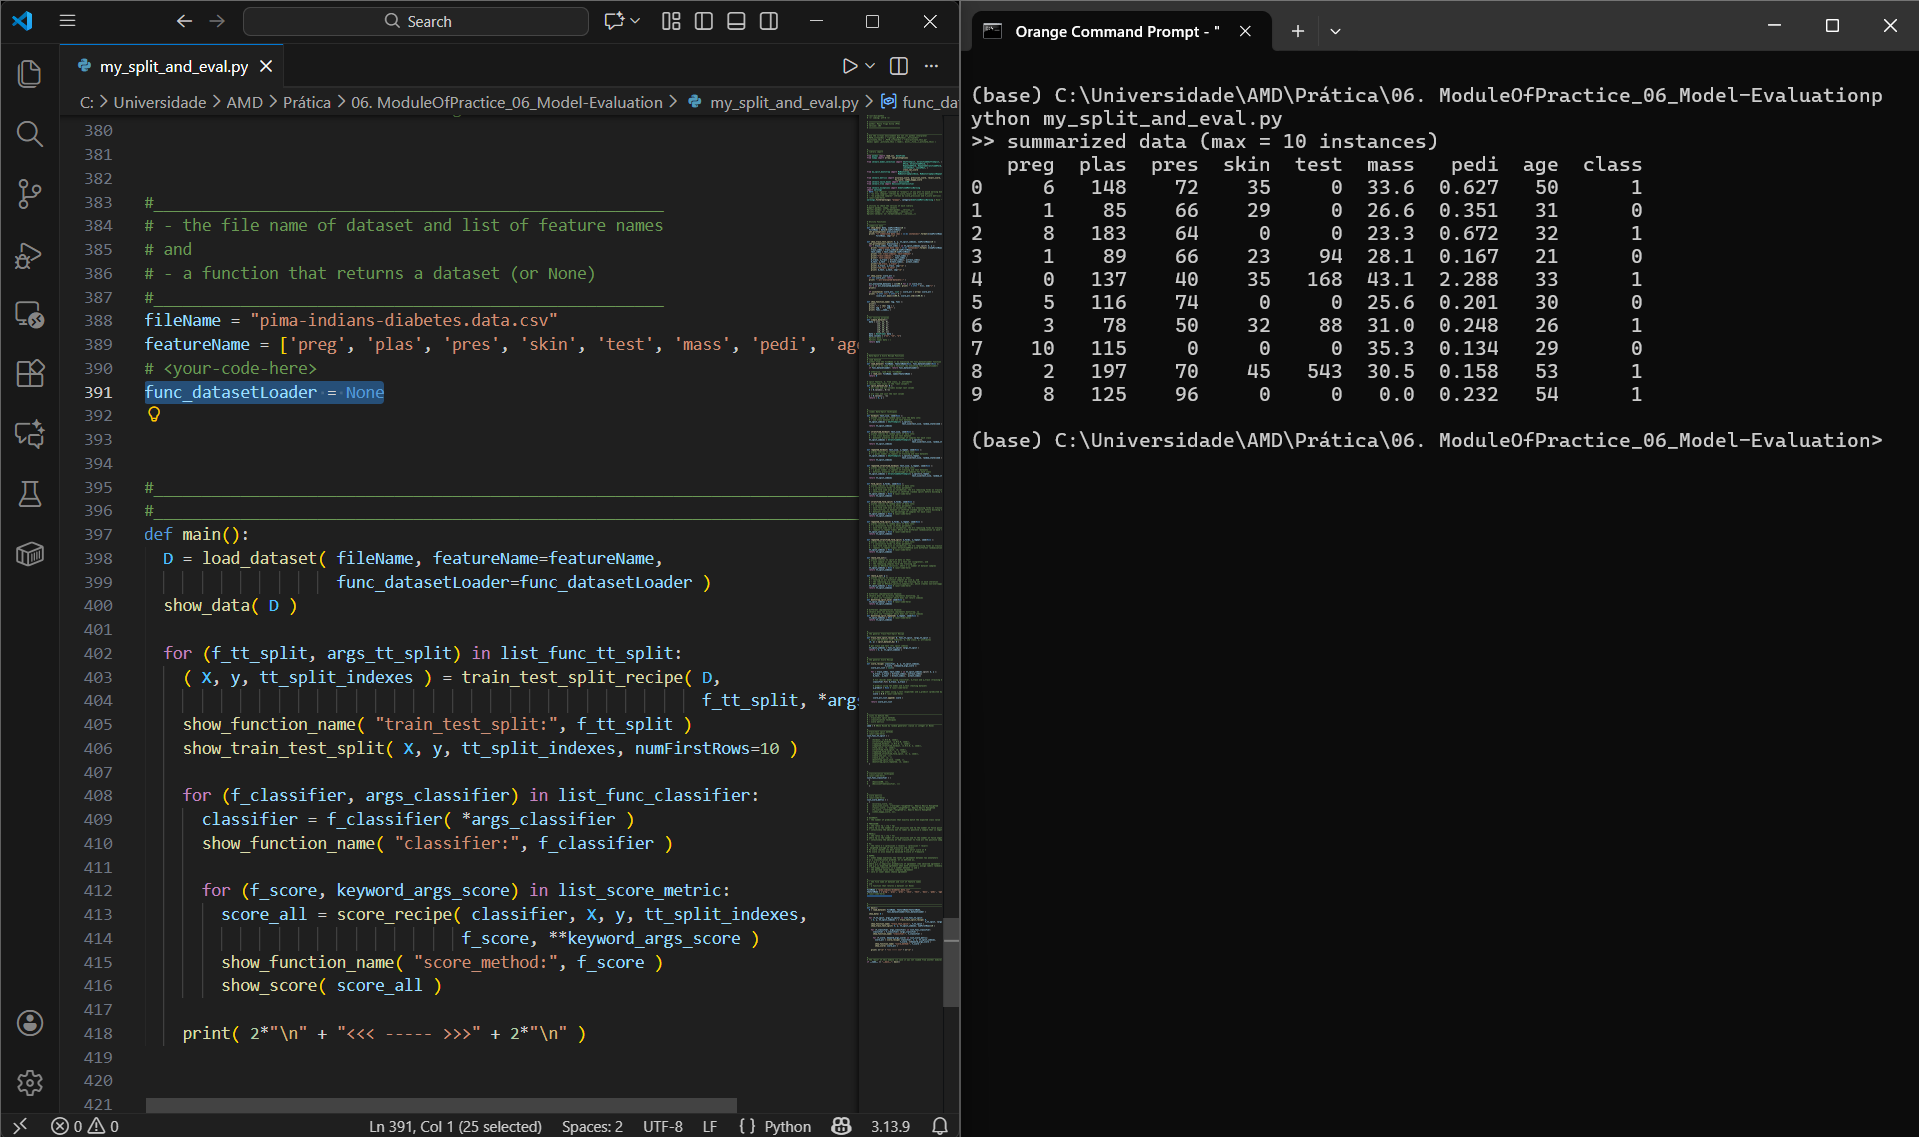
\includegraphics[width=0.9\textwidth]{figures/substituicao_simple_datas.png}
\caption{Substituição da função simple\_dataset pelo carregamento direto do dataset Pima}
\end{figure}

\subsection{2.c) Exploração da função load\_dataset}

Exploramos o funcionamento da função \texttt{load\_dataset} para compreender:
\begin{itemize}
    \item Como os dados são lidos do ficheiro CSV
    \item Como as características e labels são separadas
    \item Como os dados são convertidos para arrays NumPy
    \item Como a função lida com diferentes formatos de dados
\end{itemize}

\subsection{2.d) Retorno ao simple\_dataset}

Alteramos o mecanismo de carregamento de dados para utilizar novamente \texttt{simple\_dataset}, que fornece um conjunto de dados pequeno e controlado ideal para testes e compreensão inicial dos métodos de divisão.

\begin{figure}[H]
\centering
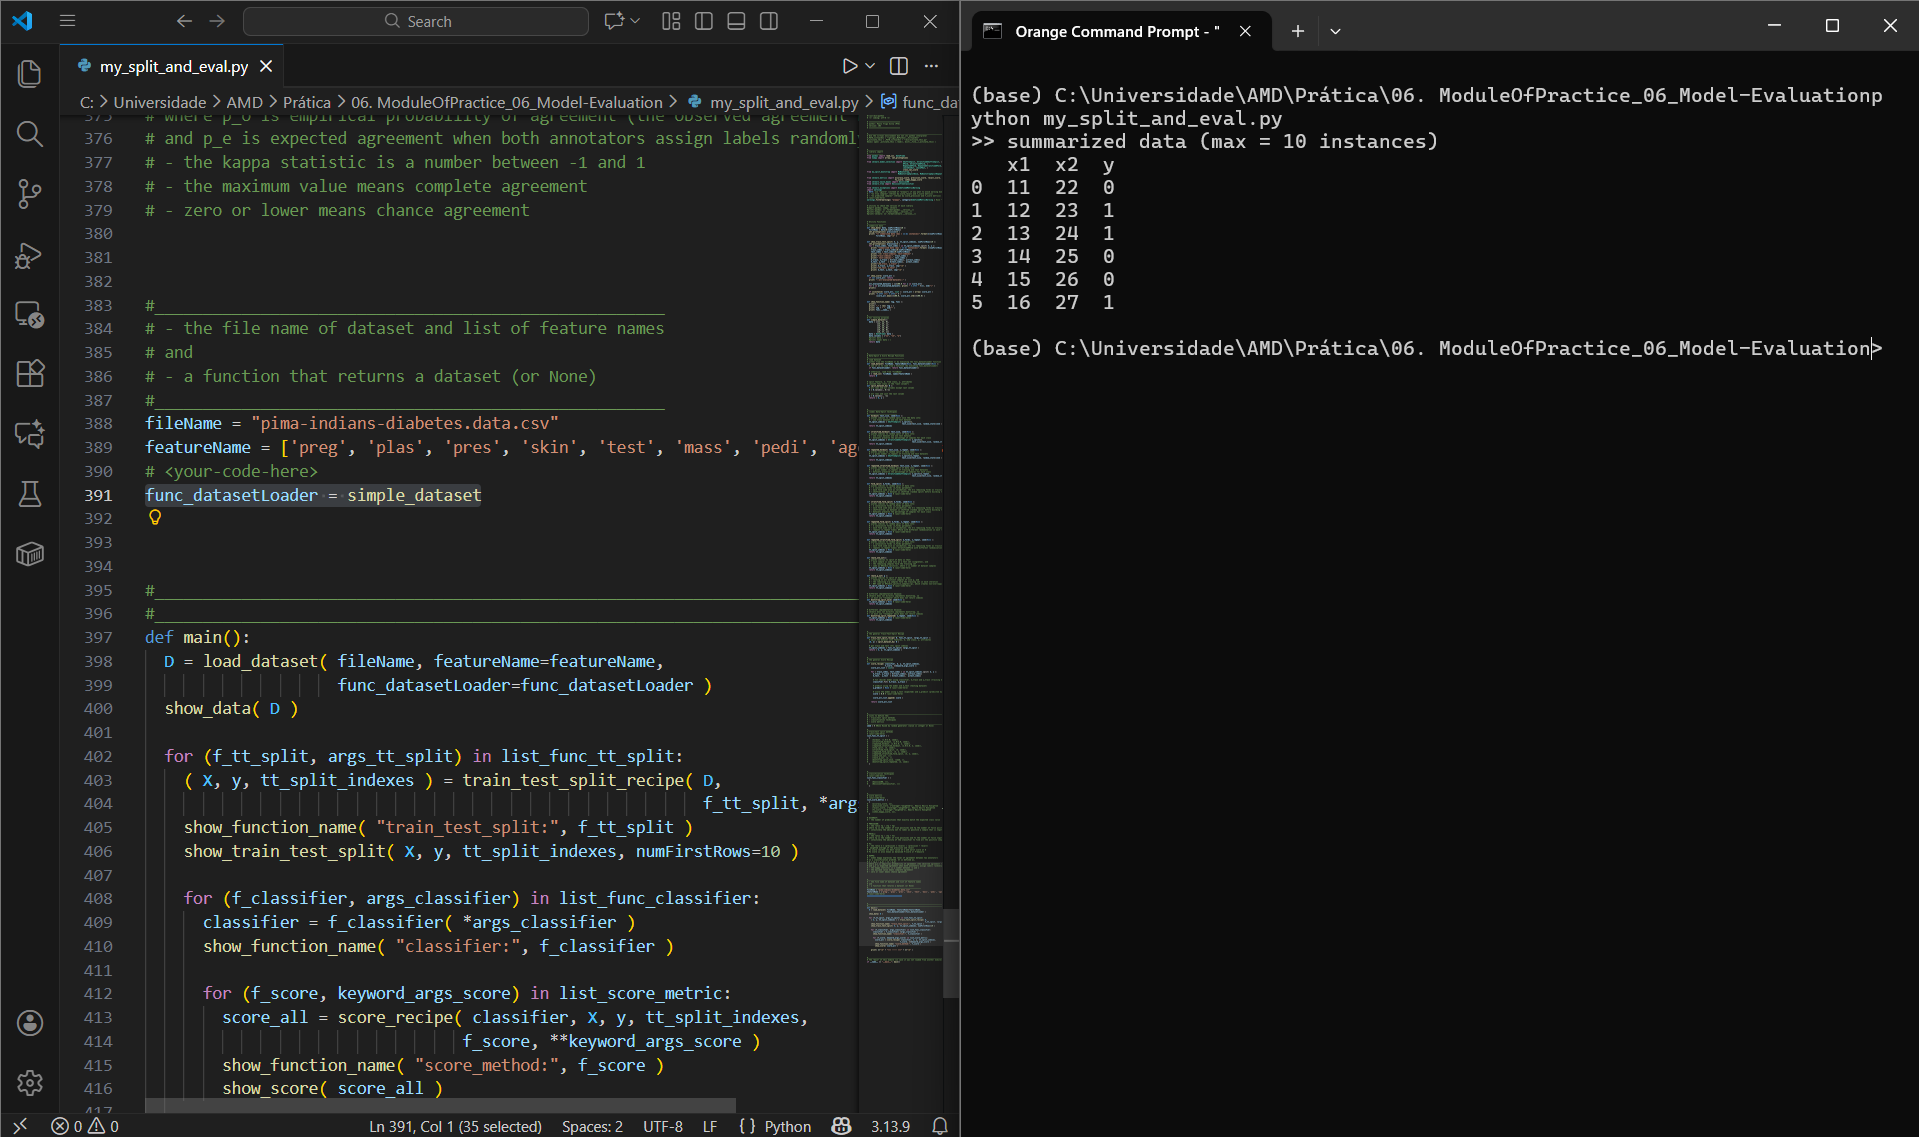
\includegraphics[width=0.9\textwidth]{figures/carregamento_dataset.png}
\caption{Carregamento do dataset simples através da função simple\_dataset}
\end{figure}

\section{Aplicação de Métodos de Separação Train-Test}

\subsection{Objetivo}

Aplicar e compreender diferentes técnicas de separação de dados em conjuntos de treino e teste, essenciais para a avaliação adequada de modelos de machine learning.

\subsection{3.a) Método Holdout}

Aplicamos o método holdout ao dataset simples fornecido pelo script. Este método divide os dados numa única vez em conjuntos de treino e teste.

\textbf{Configuração padrão:}
\begin{itemize}
    \item Proporção de teste: 1/3 (aproximadamente 33\%)
    \item Proporção de treino: 2/3 (aproximadamente 67\%)
    \item Seed aleatório para reprodutibilidade
\end{itemize}

\begin{figure}[H]
\centering
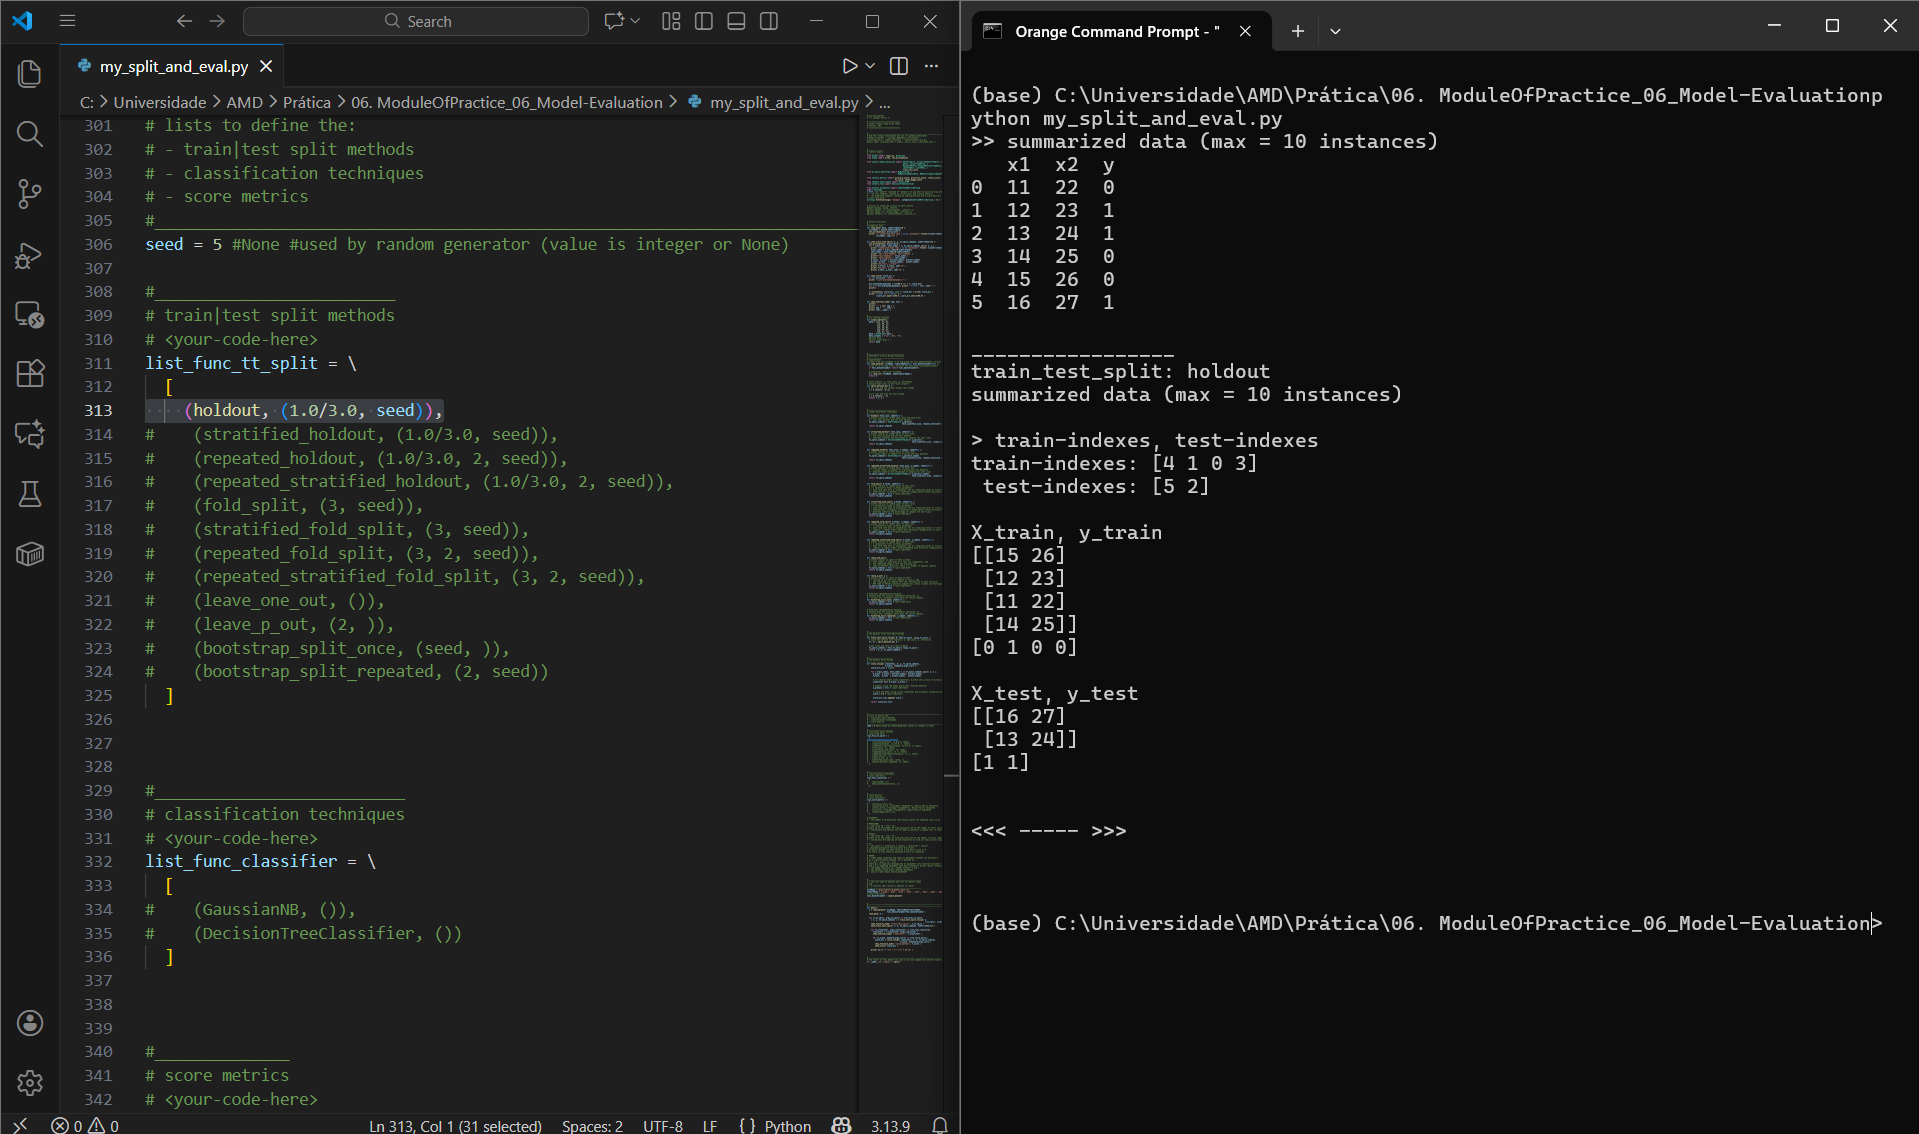
\includegraphics[width=0.9\textwidth]{figures/metodo_holdout.png}
\caption{Aplicação do método holdout ao dataset simples}
\end{figure}

\subsection{3.b) Método Holdout com Divisão 50/50}

Repetimos o método holdout, alterando o rácio para 50\% train e 50\% test. Esta configuração:
\begin{itemize}
    \item Equilibra o tamanho dos conjuntos de treino e teste
    \item Pode ser útil quando se tem dados limitados
    \item Reduz o tamanho do conjunto de treino, potencialmente afetando o desempenho do modelo
\end{itemize}

\begin{figure}[H]
\centering
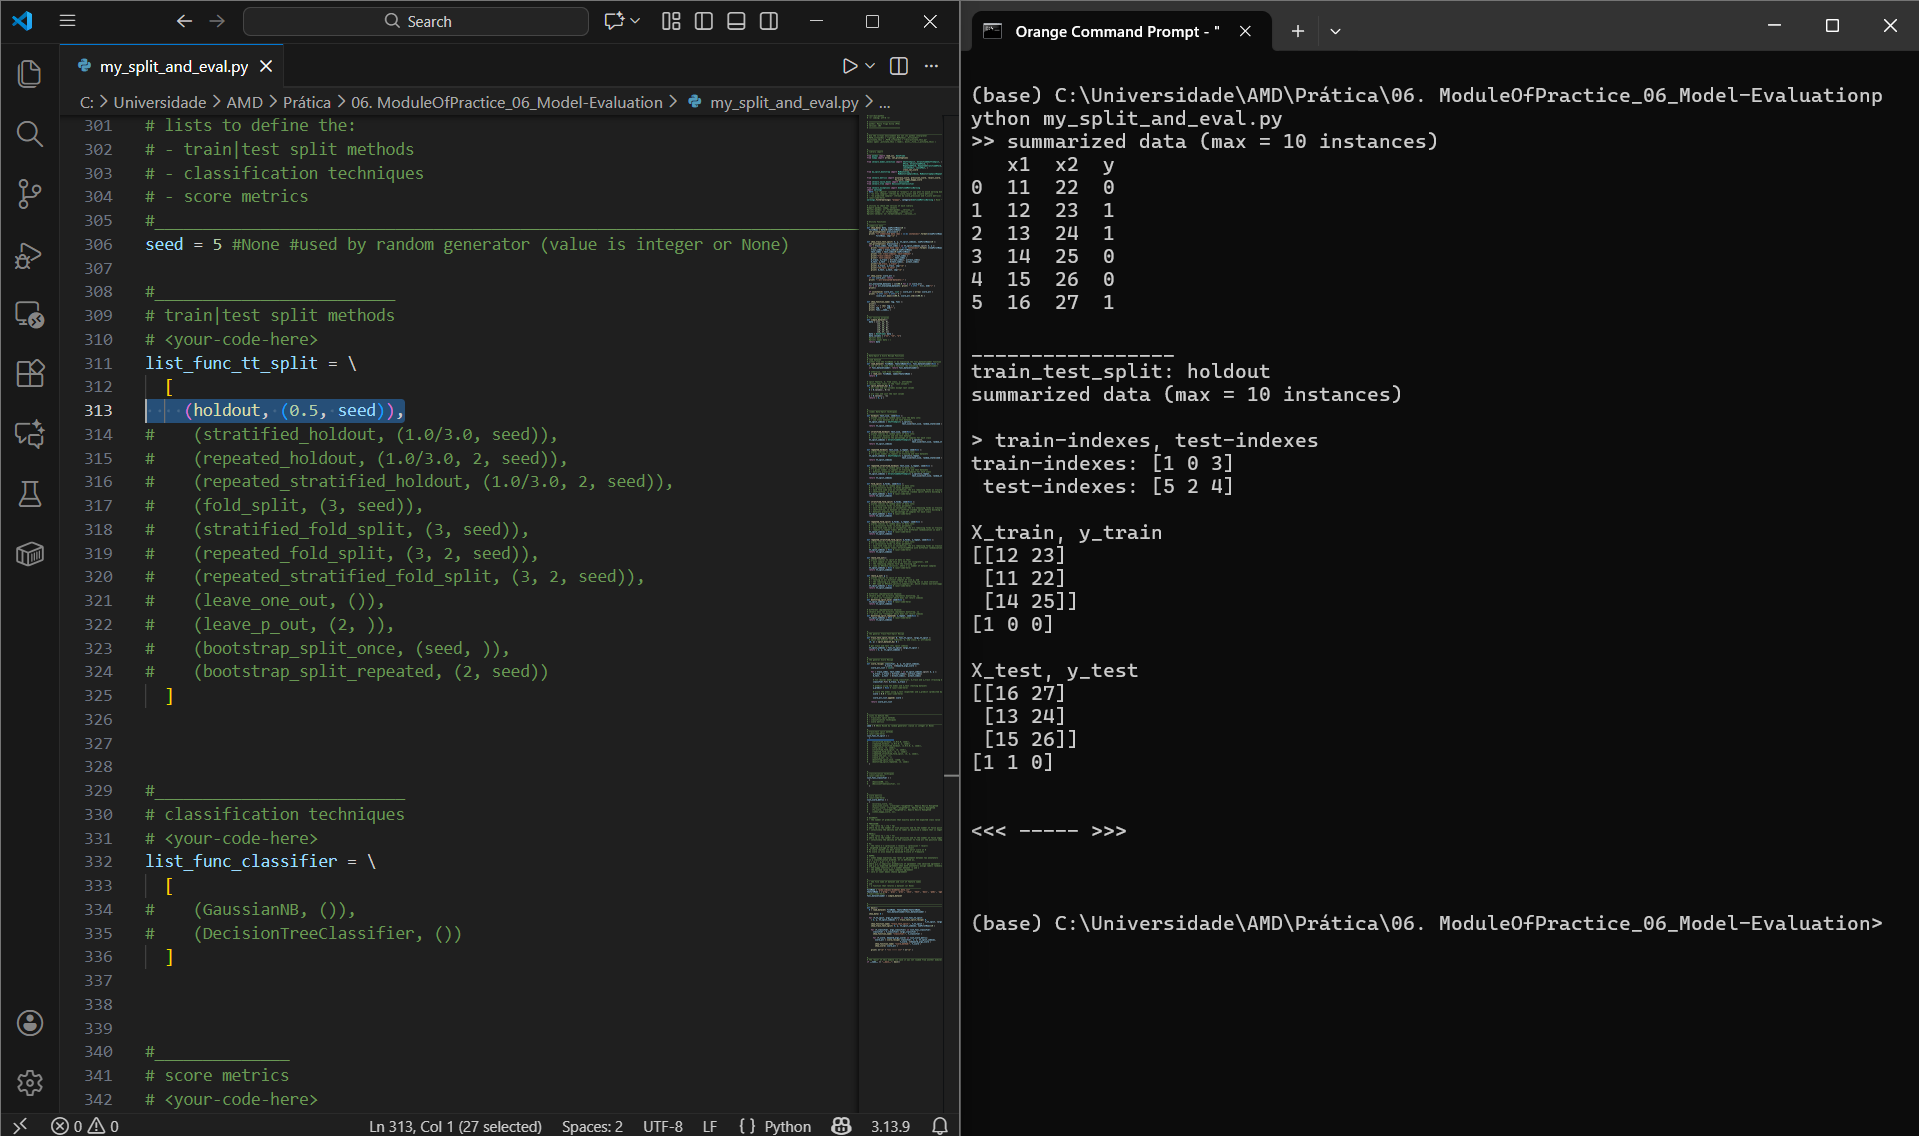
\includegraphics[width=0.9\textwidth]{figures/divisao_50_50.png}
\caption{Método holdout com divisão 50/50 aplicado ao dataset simples}
\end{figure}

\subsection{3.c) Método Stratified Holdout}

Aplicamos o método \texttt{stratified\_holdout}, que preserva a proporção das classes no processo de divisão train-test.

\textbf{Vantagens da divisão estratificada:}
\begin{itemize}
    \item Mantém a distribuição de classes em ambos os conjuntos
    \item Particularmente importante para datasets desequilibrados
    \item Reduz a variância nas estimativas de desempenho
    \item Garante que ambos os conjuntos são representativos da distribuição original
\end{itemize}

\begin{figure}[H]
\centering
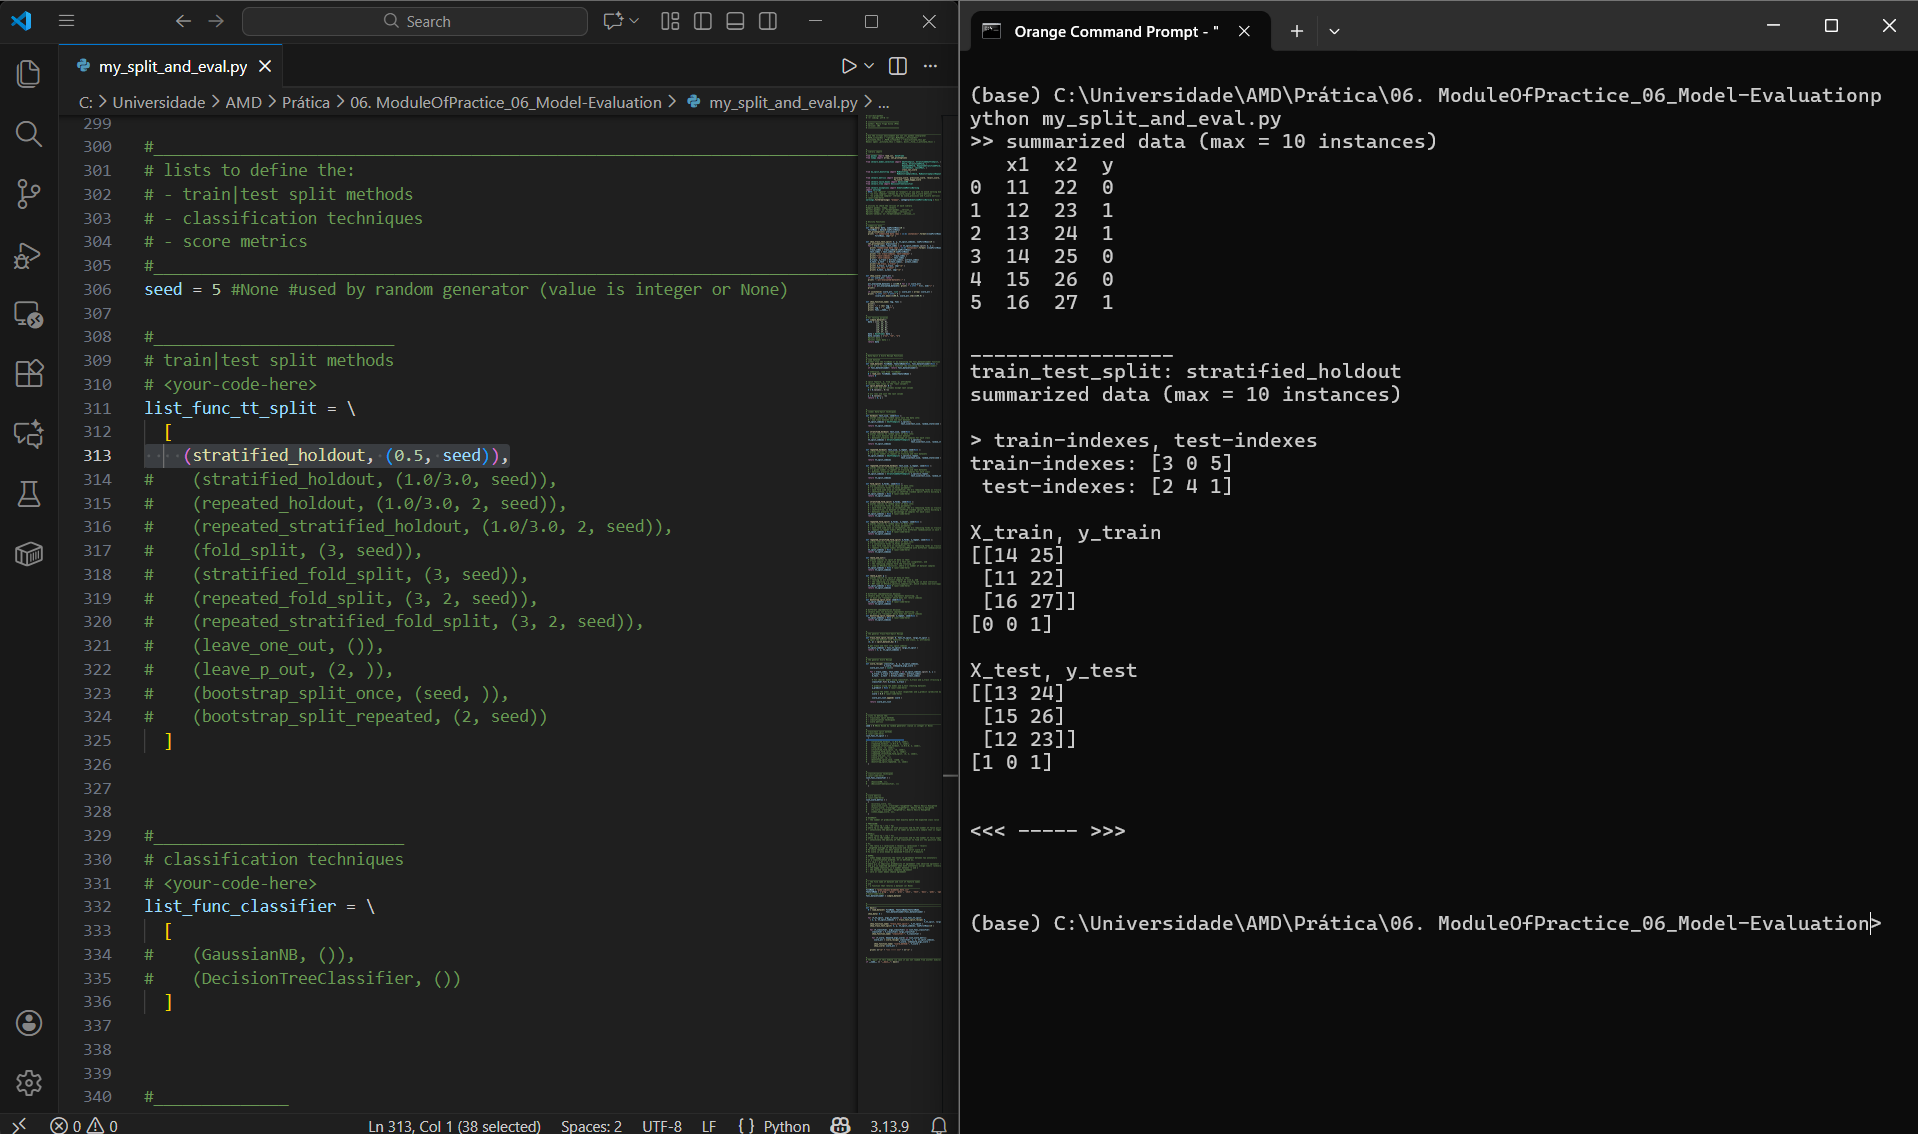
\includegraphics[width=0.9\textwidth]{figures/divisaoestratificada_50_50.png}
\caption{Divisão estratificada 50/50 preservando as proporções das classes}
\end{figure}

\subsection{3.d) Método Repeated Stratified Holdout}

Aplicamos o método \texttt{repeated\_stratified\_holdout}, que executa várias divisões estratificadas sucessivas.

\textbf{Configuração utilizada:}
\begin{itemize}
    \item Divisão 50/50
    \item 2 repetições com seeds diferentes
    \item Preservação da proporção de classes em cada repetição
\end{itemize}

\textbf{Benefícios das repetições:}
\begin{itemize}
    \item Reduz a dependência de uma única divisão aleatória
    \item Fornece múltiplas estimativas de desempenho
    \item Permite calcular média e desvio padrão das métricas
    \item Aumenta a confiança estatística nos resultados
\end{itemize}

\begin{figure}[H]
\centering
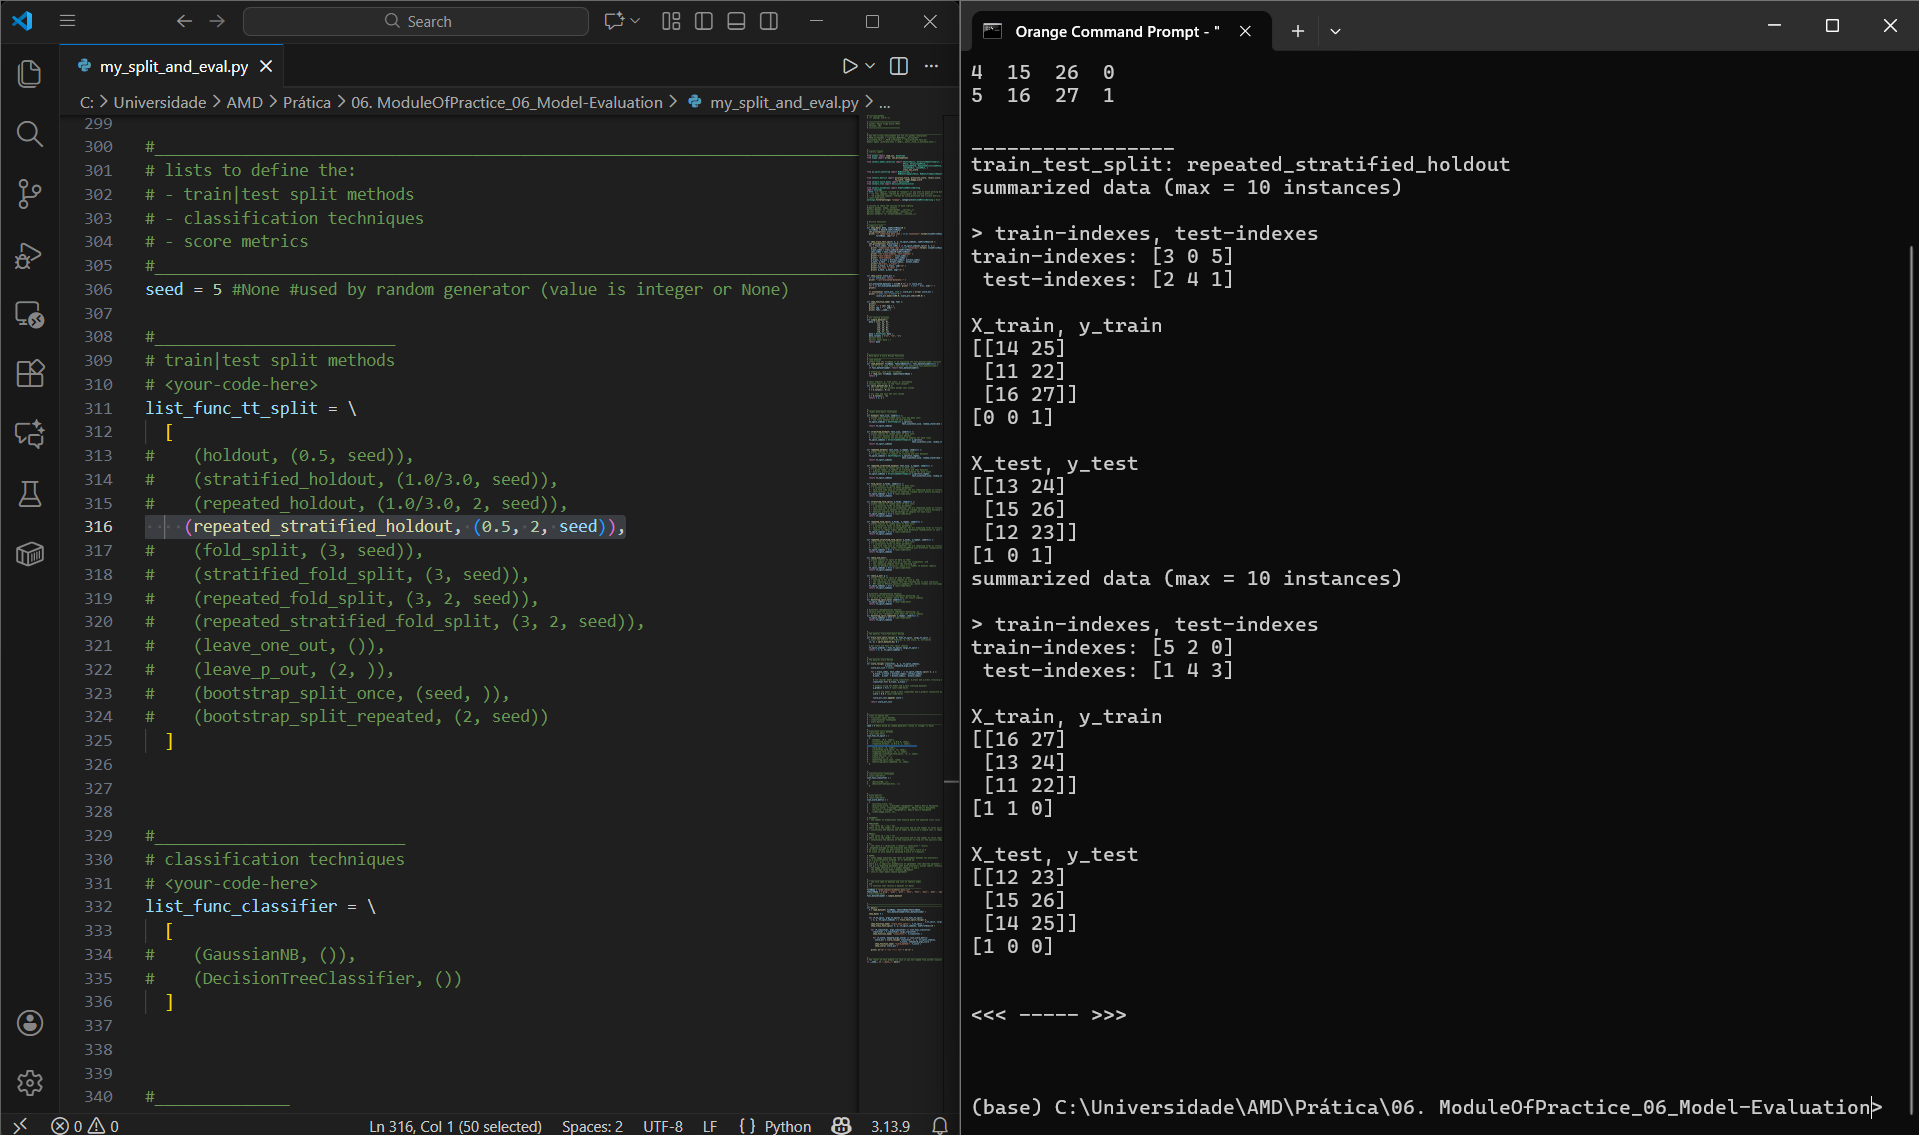
\includegraphics[width=0.9\textwidth]{figures/repeated_stratified_holdout.png}
\caption{Aplicação do método repeated\_stratified\_holdout com duas repetições}
\end{figure}

\section{Código Completo de Train-Test e Análise de Resultados}

\subsection{Objetivo}

Aprofundar as técnicas de validação, implementando vários métodos e analisando o seu comportamento em diferentes cenários.

\subsection{4.a) Implementação de Métodos Adicionais}

Todos os métodos restantes foram implementados no ficheiro \texttt{my\_split\_and\_eval.py}. Estes métodos incluem:

\begin{itemize}
    \item \textbf{leave\_one\_out:} Remove uma instância de cada vez para teste
    \item \textbf{leave\_p\_out:} Remove p instâncias de cada vez para teste
    \item \textbf{k\_fold:} Divide os dados em k partições
    \item \textbf{stratified\_k\_fold:} K-fold com preservação de proporções de classes
    \item \textbf{bootstrap:} Amostragem com reposição
\end{itemize}

\subsection{4.b) Análise de Estratégias}

Os métodos implementados cobrem um vasto leque de estratégias -- desde abordagens exaustivas, como \texttt{leave\_one\_out} e \texttt{leave\_p\_out}, até técnicas que criam múltiplas divisões com menor custo computacional, como \texttt{k\_fold} e \texttt{bootstrap}.

\textbf{Comparação de métodos:}

\begin{table}[H]
\centering
\begin{tabular}{|l|c|c|c|}
\hline
\textbf{Método} & \textbf{Custo Computacional} & \textbf{Variância} & \textbf{Uso Recomendado} \\
\hline
Holdout & Muito baixo & Alta & Datasets grandes \\
Leave-one-out & Muito alto & Muito baixa & Datasets pequenos \\
K-fold & Moderado & Moderada & Uso geral \\
Bootstrap & Configurável & Baixa & Datasets médios \\
\hline
\end{tabular}
\caption{Comparação de métodos de validação}
\end{table}

Cada método serve um propósito diferente, sendo importante considerar qual é o mais adequado para a situação específica.

\subsection{4.c) Resultados e Incompatibilidades}

As funções produziram resultados de classificação variados: algumas entregaram divisões precisas, enquanto outras não tiveram um desempenho tão bom.

\textbf{Problemas identificados:}
\begin{itemize}
    \item Certas abordagens mostraram-se incompatíveis com o dataset utilizado
    \item Os métodos \texttt{leave\_one\_out} e \texttt{leave\_p\_out} entraram em loop infinito com o dataset pequeno
    \item A incompatibilidade impediu a obtenção de resultados de classificação para estes métodos
\end{itemize}

\textbf{Lições aprendidas:}
\begin{itemize}
    \item A escolha do método de validação deve considerar o tamanho do dataset
    \item Métodos exaustivos podem ser impraticáveis para certos datasets
    \item É importante testar a viabilidade computacional antes da aplicação em produção
\end{itemize}

\section{Análise e Implementação Bootstrap}

\subsection{Objetivo}

Analisar o método bootstrap e corrigir a implementação incompleta fornecida, compreendendo os princípios da amostragem com reposição.

\subsection{5.a) Execução do Script Bootstrap}

Executamos o ficheiro \texttt{my\_split\_bootstrap.py} utilizando o VSCode. O script inicial apresentava uma implementação incompleta do método de divisão bootstrap.

\begin{figure}[H]
\centering
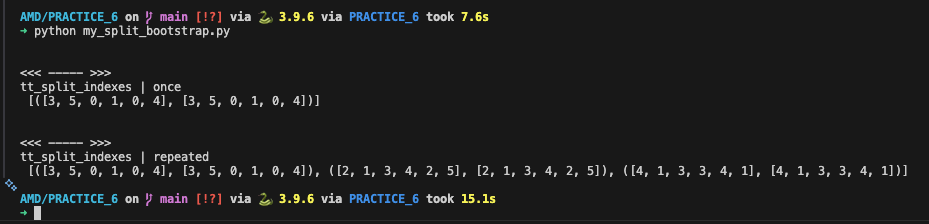
\includegraphics[width=0.9\textwidth]{figures/output_my_split_bootstrap.png}
\caption{Output da execução de my\_split\_bootstrap.py}
\end{figure}

\subsection{5.b) Correção do Conjunto de Teste}

Identificamos que o conjunto de teste deve conter apenas amostras não utilizadas no treino. Implementamos um filtro dos índices originais para manter apenas aqueles ausentes do conjunto de treino, permitindo uma avaliação adequada do modelo.

\textbf{Implementação correta:}
\begin{lstlisting}
# Filtrar indices para obter apenas amostras nao utilizadas no treino
test_indices = [i for i in range(len(X)) if i not in train_indices]
\end{lstlisting}

\textbf{Justificação:}
\begin{itemize}
    \item Garante independência entre conjuntos de treino e teste
    \item Evita sobreajuste artificial nas métricas de avaliação
    \item Mantém a integridade da validação do modelo
\end{itemize}

\begin{figure}[H]
\centering
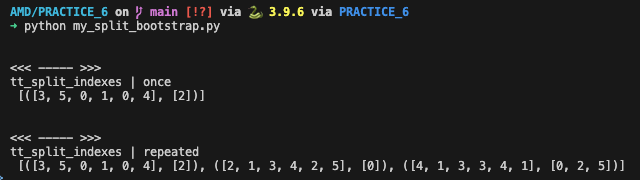
\includegraphics[width=0.9\textwidth]{figures/output_after_split.png}
\caption{Output após atualização do método de divisão}
\end{figure}

\subsection{5.c) Teste com Diferentes Repetições}

Testamos a reamostragem bootstrap com 10, 50 e 100 repetições para demonstrar como o aumento do número de divisões treino-teste fornece uma avaliação de modelo mais robusta através de múltiplas rondas independentes de validação.

\textbf{Observações:}

\begin{table}[H]
\centering
\begin{tabular}{|c|c|c|}
\hline
\textbf{Repetições} & \textbf{Tempo de Execução} & \textbf{Estabilidade} \\
\hline
10 & Rápido & Moderada \\
50 & Moderado & Boa \\
100 & Mais lento & Muito boa \\
\hline
\end{tabular}
\caption{Impacto do número de repetições bootstrap}
\end{table}

\begin{itemize}
    \item Maior número de repetições aumenta a confiança estatística
    \item Existe um compromisso entre precisão e custo computacional
    \item Para datasets médios, 50-100 repetições são geralmente suficientes
\end{itemize}

\begin{figure}[H]
\centering
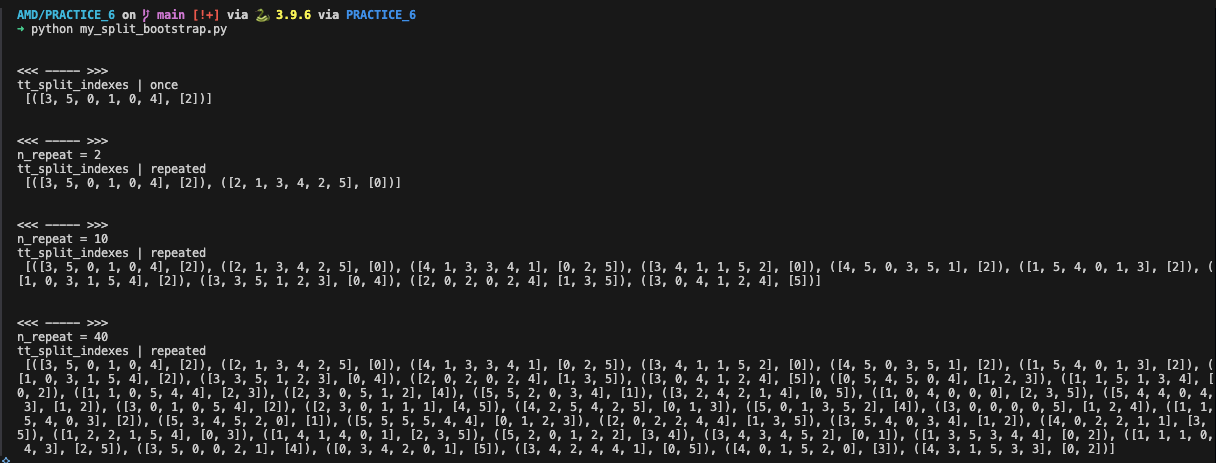
\includegraphics[width=0.9\textwidth]{figures/output_repetitions.png}
\caption{Output com diferentes números de repetições (10, 50, 100)}
\end{figure}

\subsection{5.d) Integração no Script Principal}

Implementamos métodos de divisão treino-teste bootstrap criando instâncias das classes \texttt{MyBootstrapSplitOnce} e \texttt{MyBootstrapSplitRepeated}, já importadas no início do ficheiro, permitindo reamostragem bootstrap simples e repetida para avaliação de modelos.

\textbf{Integração no \texttt{my\_split\_and\_eval.py}:}
\begin{lstlisting}
# Bootstrap simples
("bootstrap_once", MyBootstrapSplitOnce(), ()),

# Bootstrap repetido
("bootstrap_repeated", MyBootstrapSplitRepeated(n_repeats=50), ()),
\end{lstlisting}

\section{Construir um Classificador com Divisão Treino-Teste}

\subsection{Exercício 6 (b): Aplicar o DecisionTreeClassifier}

O exercício solicita procurar a tag \texttt{<your-code-here>} e aplicar o \texttt{DecisionTreeClassifier}. Ao executar o código inicial, observámos que "nada aconteceu" porque, embora o classificador tenha sido criado, nenhum método de divisão treino-teste estava ativo para treinar e avaliar o modelo.

\subsubsection{Implementação}

Na lista de classificadores (linhas 354-358), ativamos o \texttt{DecisionTreeClassifier}:
\begin{lstlisting}[language=Python]
list_func_classifier = \
  [
#    (GaussianNB, ()),
   (DecisionTreeClassifier, ())
  ]
\end{lstlisting}

Esta configuração é utilizada na função \texttt{main()} (linha 409) onde o classificador é instanciado:
\begin{lstlisting}[language=Python]
classifier = f_classifier( *args_classifier )
\end{lstlisting}

Que resulta em \texttt{classifier = DecisionTreeClassifier()}.

Sem um método de divisão treino-teste ativo na lista \texttt{list\_func\_tt\_split}, o classificador não é treinado nem avaliado, resultando em nenhuma saída visível no terminal.

\subsection{Exercício 6 (c): Aplicar a Divisão Holdout}

O próximo passo foi ativar o método de divisão treino-teste \texttt{holdout} (utilizando \texttt{DecisionTreeClassifier}). Ao executar o código, observámos que agora é necessário aplicar a função \texttt{score\_recipe} utilizando algum(ns) método(s) de pontuação para avaliar o desempenho do modelo.

\subsubsection{Implementação}

Na lista de métodos de divisão (linhas 328-341), ativamos o método \texttt{holdout}:
\begin{lstlisting}[language=Python]
list_func_tt_split = \
  [
   (holdout, (1.0/3.0, seed)),
#    (stratified_holdout, (1.0/3.0, seed)),
#    (repeated_holdout, (1.0/3.0, 2, seed)),
#    ...
  ]
\end{lstlisting}

Isto configura uma divisão holdout com 1/3 dos dados para teste (aproximadamente 33\%) e 2/3 para treino (aproximadamente 67\%), utilizando \texttt{seed=5} para reprodutibilidade.

\subsubsection{Método de Divisão Holdout}

O método holdout é a abordagem mais simples para divisão treino-teste. Divide o conjunto de dados numa única vez em dois subconjuntos:

\begin{itemize}
    \item \textbf{Conjunto de Treino:} Utilizado para treinar o modelo (tipicamente 60-80\% dos dados)
    \item \textbf{Conjunto de Teste:} Utilizado para avaliar o desempenho do modelo (tipicamente 20-40\% dos dados)
\end{itemize}

\textbf{Vantagens do Holdout:}
\begin{itemize}
    \item Computacionalmente eficiente (apenas uma divisão)
    \item Simples de implementar e compreender
    \item Adequado para conjuntos de dados grandes
\end{itemize}

\textbf{Desvantagens do Holdout:}
\begin{itemize}
    \item Alta variância nos resultados (dependente da divisão específica)
    \item Pode não ser representativo para conjuntos de dados pequenos
    \item Utiliza menos dados para treino em comparação com validação cruzada
\end{itemize}

\subsubsection{Implementação}

No código fornecido, o método holdout está configurado como:
\begin{lstlisting}
( "holdout", holdout, (1.0/3.0, 5) ),
\end{lstlisting}

Isto configura:
\begin{itemize}
    \item \textbf{Proporção de teste:} 1/3 (aproximadamente 33\%) dos dados para teste
    \item \textbf{Proporção de treino:} 2/3 (aproximadamente 67\%) dos dados para treino
    \item \textbf{Seed aleatório:} 5 (para reprodutibilidade)
\end{itemize}

\subsubsection{Classificador: Árvore de Decisão}

O exercício utiliza o \texttt{DecisionTreeClassifier} do scikit-learn. As árvores de decisão são uma escolha popular devido à sua:
\begin{itemize}
    \item Interpretabilidade (estrutura em árvore visualizável)
    \item Capacidade de lidar com características numéricas e categóricas
    \item Não necessidade de normalização de características
    \item Capacidade de capturar relações não-lineares
\end{itemize}

\subsubsection{Conjunto de Dados: Pima Indians Diabetes}

O conjunto de dados utilizado contém:
\begin{itemize}
    \item \textbf{Instâncias:} 768 pacientes
    \item \textbf{Características:} 8 características médicas (gravidez, glucose, pressão arterial, etc.)
    \item \textbf{Classes:} 2 (diabético vs. não-diabético)
    \item \textbf{Distribuição:} 268 positivos (34.9\%), 500 negativos (65.1\%)
\end{itemize}

\subsubsection{Resultados}

Ao executar o script com apenas o método holdout ativo, obtivemos:

\begin{table}[H]
\centering
\begin{tabular}{|l|c|}
\hline
\textbf{Métrica} & \textbf{Valor} \\
\hline
Exatidão (Accuracy) & 66.15\% \\
\hline
\end{tabular}
\caption{Resultados do Exercício 6 utilizando divisão holdout}
\end{table}

\textbf{Interpretação dos Resultados:}

\begin{itemize}
    \item A exatidão de 66.15\% significa que o classificador prevê corretamente a classe para aproximadamente 2 em cada 3 instâncias
    \item Este valor está acima do baseline de classe maioritária (65.1\%), indicando que o modelo aprendeu alguns padrões
    \item No entanto, há espaço significativo para melhoria, possivelmente através de:
    \begin{itemize}
        \item Ajuste de hiperparâmetros da árvore de decisão
        \item Engenharia de características
        \item Tentativa de diferentes algoritmos de classificação
        \item Tratamento de valores em falta ou outliers
    \end{itemize}
\end{itemize}

\section{Múltiplas Métricas e Divisões Repetidas}

\subsection{(d) Completar a Função score\_recipe}

Procurámos a tag \texttt{<your-code-here>} na função \texttt{score\_recipe} (linhas 296-314) e completámos o código:

\begin{lstlisting}[language=Python]
# predict using the model and X_test (testing dataset)
y_predict = classifier.predict( X_test )

# score the model using y_test (expected) and y_predict (predicted by model)
score = f_score( y_test, y_predict, **keyword_args_score )
\end{lstlisting}

\vspace{2cm}

\subsection{(e) Testar o Código}

Testámos o código com a configuração especificada: \texttt{repeated\_holdout(1.0/3.0, 2, seed)} e \texttt{DecisionTreeClassifier} com \texttt{seed=5}.

Resultados obtidos:

\begin{lstlisting}
score_method: accuracy_score
::all-evaluated-datasets::
50.00% | 0.00% |
25.00% (+/- 25.00%)

score_method: precision_score
::all-evaluated-datasets::
100.00% | 0.00% |
50.00% (+/- 50.00%)

score_method: recall_score
::all-evaluated-datasets::
50.00% | 0.00% |
25.00% (+/- 25.00%)

score_method: f1_score
::all-evaluated-datasets::
66.67% | 0.00% |
33.33% (+/- 33.33%)

score_method: cohen_kappa_score
::all-evaluated-datasets::
0.00% | 0.00% |
0.00% (+/- 0.00%)
\end{lstlisting}

\subsection{(f) Observar os Avisos}

Durante a execução, surgiram avisos (warnings). Identificámos os seguintes textos importantes:

\textbf{Aviso "no predicted samples":}
\begin{lstlisting}
UndefinedMetricWarning: Precision is ill-defined and being set to 0.0 
due to no predicted samples.
\end{lstlisting}

\textbf{Aviso "no true samples":}
\begin{lstlisting}
UndefinedMetricWarning: Recall is ill-defined and being set to 0.0 
due to no true samples.
\end{lstlisting}

\subsection{(g) Explicar a Diferença entre Avisos}

\subsubsection{Diferença entre Avisos}

\textbf{"no predicted samples":}
\begin{itemize}
    \item Significa que o classificador não previu nenhuma instância como positiva (TP + FP = 0)
    \item Todas as previsões foram da classe negativa
    \item Afeta a métrica de precisão (precision)
\end{itemize}

\textbf{"no true samples":}
\begin{itemize}
    \item Significa que o conjunto de teste não contém nenhuma instância positiva verdadeira (TP + FN = 0)
    \item Todas as instâncias reais no conjunto de teste são da classe negativa
    \item Afeta a métrica de revocação (recall)
\end{itemize}

\subsubsection{Aviso: no true samples (recall e f1-score)}

A revocação (recall) é definida como:
\begin{equation}
\text{Recall} = \frac{TP}{TP + FN}
\end{equation}

Quando não há amostras verdadeiras positivas no conjunto de teste, temos TP + FN = 0, o que resulta em divisão por zero. O F1-score depende de recall, portanto herda este problema.

\subsubsection{Aviso: no predicted samples (precision e f1-score)}

A precisão (precision) é definida como:
\begin{equation}
\text{Precision} = \frac{TP}{TP + FP}
\end{equation}

Quando o classificador não prevê nenhuma amostra como positiva, temos TP + FP = 0, o que resulta em divisão por zero. O F1-score depende de precision, portanto herda este problema.

\subsection{(h) Utilizar o Parâmetro zero\_division}

Lemos a documentação do scikit-learn para as funções \texttt{precision\_score} e \texttt{recall\_score}. Utilizámos o parâmetro \texttt{zero\_division} para eliminar os avisos.

Na lista de métricas (linhas 365-373):

\begin{lstlisting}[language=Python]
list_score_metric = \
  [
   (accuracy_score, {}),
   (precision_score, {"average":"weighted", "zero_division":0}),
   (recall_score, {"average":"weighted", "zero_division":0}),
   (f1_score, {"average":"weighted", "zero_division":0}),
   (cohen_kappa_score, {}),
  ]
\end{lstlisting}

O parâmetro \texttt{zero\_division=0} define o valor da métrica como 0.0 quando ocorre divisão por zero, eliminando os avisos.

\subsection{(i) Desativar Avisos UndefinedMetricWarning}

Procurámos a tag \texttt{<your-code-here>} e utilizámos o valor "ignore" para desativar a apresentação de avisos da categoria \texttt{UndefinedMetricWarning}.

No início do ficheiro (linhas 39-43):

\begin{lstlisting}[language=Python]
from sklearn.exceptions import UndefinedMetricWarning
import warnings

warnings.filterwarnings( "ignore", category=UndefinedMetricWarning )
\end{lstlisting}

\textbf{Aviso importante:} Ao desativar estes avisos, perde-se informação importante sobre problemas no conjunto de dados ou no modelo. Só se deve fazer isto quando realmente se conhece o impacto correspondente!

\section{Conclusão}

A realização deste laboratório permitiu percorrer todas as etapas de avaliação de modelos preditivos: preparação do ambiente, carregamento de dados, divisão correta de test-train, implementação de métodos avançados de amostragem e integração de métricas de desempenho.

\subsection{Competências Adquiridas}

Ao longo dos sete exercícios, desenvolvemos competências em:

\begin{enumerate}
    \item \textbf{Preparação de Ambiente:} Integração de bibliotecas Python (pandas, numpy, scikit-learn) no ambiente Orange Data Mining
    
    \item \textbf{Gestão de Dados:} Carregamento e processamento de datasets reais (Pima Indians Diabetes) e sintéticos
    
    \item \textbf{Métodos de Validação:} Implementação e comparação de múltiplos métodos de divisão treino-teste:
    \begin{itemize}
        \item Holdout simples e estratificado
        \item Holdout repetido
        \item Leave-one-out e leave-p-out
        \item K-fold e stratified k-fold
        \item Bootstrap simples e repetido
    \end{itemize}
    
    \item \textbf{Construção de Classificadores:} Implementação de árvores de decisão com scikit-learn
    
    \item \textbf{Avaliação de Desempenho:} Aplicação de múltiplas métricas (exatidão, precisão, revocação, F1-score, Kappa de Cohen)
    
    \item \textbf{Análise Crítica:} Interpretação de avisos, identificação de limitações e gestão de casos extremos
\end{enumerate}

\subsection{Principais Aprendizagens}

\begin{itemize}
    \item \textbf{Tamanho do dataset importa:} Conjuntos de dados pequenos levam a métricas não fiáveis e avisos frequentes
    
    \item \textbf{Múltiplas métricas são essenciais:} Exatidão por si só pode ser enganadora; precisão, revocação e F1-score fornecem visão completa
    
    \item \textbf{Escolha adequada do método:} Cada técnica de validação tem o seu caso de uso ideal, considerando tamanho do dataset e custo computacional
    
    \item \textbf{Estratificação é crucial:} Preservar proporções de classes melhora significativamente a qualidade da validação
    
    \item \textbf{Repetições aumentam robustez:} Múltiplas divisões fornecem estimativas mais estáveis e confiáveis
    
    \item \textbf{Bootstrap é versátil:} A amostragem com reposição oferece um bom compromisso entre precisão e eficiência
    
    \item \textbf{Tratamento de avisos:} Compreender os avisos de métricas indica problemas de dados reais, não apenas questões técnicas
\end{itemize}

\subsection{Visão Final}

No final, o laboratório fornece uma visão completa das práticas recomendadas para avaliar modelos de Machine Learning de forma rigorosa. A experiência demonstra que a avaliação adequada de classificadores requer:

\begin{itemize}
    \item Conjuntos de dados de tamanho suficiente para validação robusta
    \item Múltiplas perspetivas através de diferentes métricas
    \item Compreensão profunda das limitações de cada método e métrica
    \item Tratamento cuidadoso de casos extremos e avisos
    \item Múltiplas avaliações para estimativas estáveis e confiáveis
    \item Escolha informada do método de validação baseada no contexto do problema
\end{itemize}

Estes exercícios estabelecem uma base sólida para técnicas de avaliação mais avançadas e para a aplicação prática de machine learning em problemas reais, garantindo que os modelos desenvolvidos são devidamente validados e têm desempenho confiável em dados não vistos.

\end{document}
